\documentclass{standalone}

\usepackage{tikz}
\usetikzlibrary{calc,shapes.multipart,chains,arrows,positioning}
\tikzset{
    squarecross/.style={
        draw, rectangle,minimum size=18pt, fill=orange!80,
        inner sep=0pt, text=black,
        path picture = {
            \draw[black]
            (path picture bounding box.north west) -- 
            (path picture bounding box.south east)
            (path picture bounding box.south west) -- 
            (path picture bounding box.north east);
        }
    }
}

\begin{document}
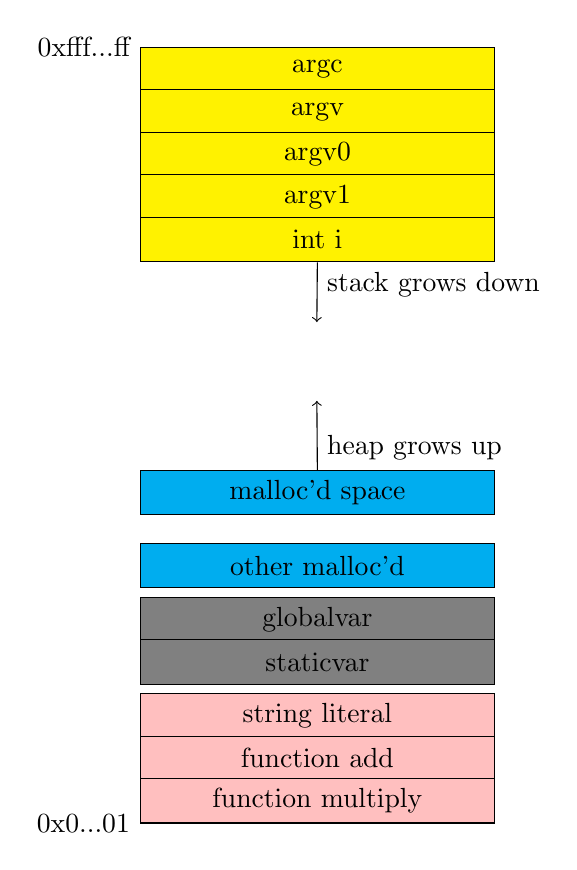
\begin{tikzpicture}[
        mem/.style={align=left,anchor=north west,minimum width=128pt,minimum height=16pt,draw,node distance=-1pt},
        stack/.style={mem,fill=yellow},
        heap/.style={mem,fill=cyan},
        global/.style={mem,fill=gray},
        code/.style={mem,fill=pink}
      ]


  \node   (argc) [stack] {argc};
  \node at (argc.north west) [anchor=east] {0xfff...ff};
  \node   (argv) [stack,below=of argc] {argv};
  \node   (argv0) [stack,below=of argv] {argv0};
  \node   (argv1) [stack,below=of argv0] {argv1};
  \node   (stackbottom) [stack,below=of argv1] {int i};
  \draw[->] (stackbottom.south) -- (2.25,-3.5) coordinate (x axis);
  \node at (stackbottom.south) [anchor=north west] {stack grows down};

  
  \node   (mallocd) [heap,below=75pt of stackbottom] {malloc'd space};
  \draw[->] (mallocd.north) -- (2.25,-4.5) coordinate (x axis);
  \node at (mallocd.north) [anchor=south west] {heap grows up};
  
  \node   (othermallocd) [heap,below=10pt of mallocd] {other malloc'd};

  \node   (global) [global,below=3pt of othermallocd] {globalvar};
  \node   (static) [global,below=of global] {staticvar};

  \node   (literal) [code,below=3pt of static] {string literal};
  \node   (func) [code,below=of literal] {function add};
  \node   (func2) [code,below=of func] {function multiply};
  \node at (func2.south west) [anchor=east] {0x0...01};


\end{tikzpicture}
\end{document}